% !TEX encoding = UTF-8 Unicode
%!TEX root = thesis.tex
% !TEX spellcheck = en-US
%%=========================================
\chapter{Visualization}

%%=========================================
\section{Design Criteria} % (fold)
\label{sub:prototype}
%After analyzing the problem at hand and the related work, we arrived
%to the following list of criteria to be followed in this project
%\marginpar{References?}:
%\begin{itemize}
%	\item Display both general and detailed information of the matching results.
%%	\item Provide intuitive display for large ontologies.
%	\item Reveal the difference between matching algorithms.
%	\item Enable user feedback acquisition.
%\end{itemize}

We have made the following choices and present their
rationale:

\begin{itemize}
  \item We do not display all the mappings at once. If we did so, it
    would be difficult to find a visualization whose size does not
    depend on the number of mappings or on the size of the ontologies
    involved.
  \item To supplement the detailed view, we allow for ontology navigation, exploration and searching.
\item We want to focus on the mappings one level at a time and
  aggregate the results for the children of the nodes at that level. As long as navigation and searching functions are available, users can easily locate any single ontology node in the whole structure and see the mappings they need.
\item We chose a visualization based on pie charts. The reason of this
  choice is that
no matter how large the data size is, the pie chart requires always
the same modest area. Given this, we can display the results of more
than one matching algorithm at a time.
\item When matching two classes, the most valuable information is the
  similarity value found by the matching algorithm. The visualization
  can give priority to those mappings that maximize the similarity
  value between two nodes.
\item We want to make apparent the differences between matching
  algorithms.
\item We enable user feedback acquisition.
\end{itemize}

%Taking into account that we want to display the matching results for
%all kinds of ontologies, including very large ones, and that we do
%not want the size of the display to grow with the size of the
%ontologies, we need to select the information that is most valuable
%and whose size will not vary depending on the size of the ontologies. 

%One of the main principles to be followed for the visualization of
%large ontologies consists of reduce the amount of data every time we represent information to users. In other words, we need to present the most valuable data within a certain size. So we consider to provide general processed information instead of raw results. Furthermore, consider that users do not need so much information at one time, we show the results level by level. As long as navigation and searching functions are available, users can easily locate any single ontology node in the whole structure and see the result they need.

%The information we use here is the matching similarity confidence,
%represented by a pie chart. The reason of using the pie chart is
%that, no matter how large the data size is, the pie chart requires
%only a small area. In addition, this feature proved to be an advantage then comparing performances of different algorithms.

\section{Pie Chart Visualization}

We start by describing how we visualize the information in terms of pie
charts. For each visualization there are two pie charts, when
corresponding to a source node $S$, called the {\it current node\/},
and a pie chart corresponding to a target node $T$. We show the
percentage of their children
whose matching similarity falls in a particular
range. Figure~\ref{fig:proto_pie} shows those ranges, namely
81\%-100\%, 61\%-80\%, 41\%-60\%, and $\le$40\%. %\marginpar{This needs to be corrected.} For a source node $S$, we show the percentage of its
%children whose matching similarity falls in the corresponding
%range. 
For example, 41\% of the children nodes of $S$ have matching
similarity values in the range 81\%-100\%. Figure~\ref{fig:proto_pie}
also highlights a mapping between two nodes, $A$ that is a child of
$S$ and $B$ that is a child of $T$. 

%fall in the respective In the right pie chart, for the target node
%$T$ that is matched to $S$, we use a similar pie chart for its
%children. These two pie charts are centered around two classes, $A$
%and $B$, belonging respectively to $S$ and $T$, and the mapping
%between them. The focus of this visualization is therefore the
%mapping between $A$ and $B$, and $A$ is the {\it current class}.
\begin{figure}[htb]
	\centering
	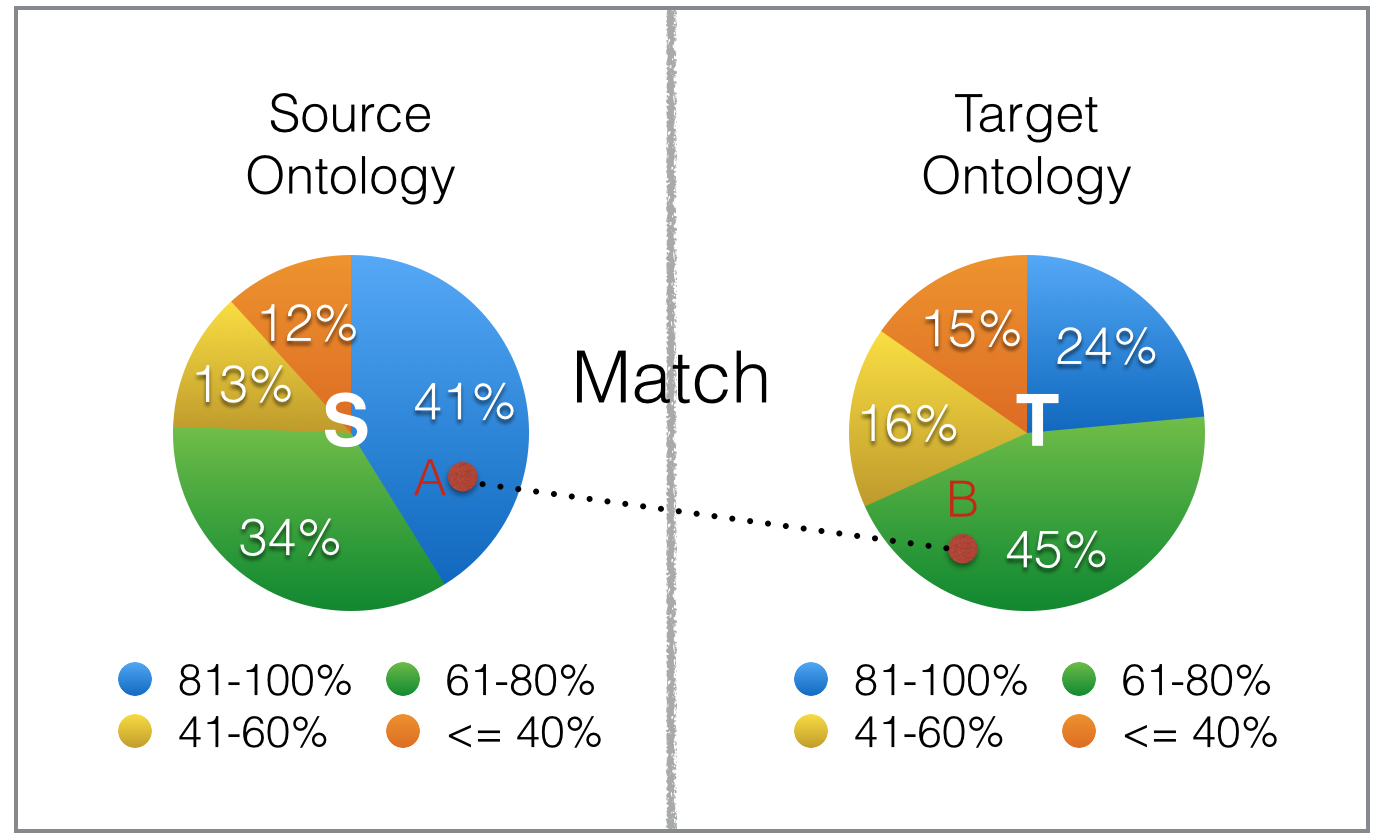
\includegraphics[width=3.5in]{pics/proto_pie.png}
	\caption{User interface prototype that displays matching results.}
	\label{fig:proto_pie}
\end{figure}
	
Figure~\ref{fig:proto_tree} shows schematically subgraphs of both
ontologies with roots $S$ and $T$, their children, among which there
are subclasses $A$ and $B$, the siblings of $A$ and $B$, and their
children (and grandchildren). To
enable navigation along the ontologies, users should be able to
traverse the ontology ``vertically'' from parents to children but also
``horizontally'' from a node to its siblings. 

\begin{figure}[htb]
	\centering
	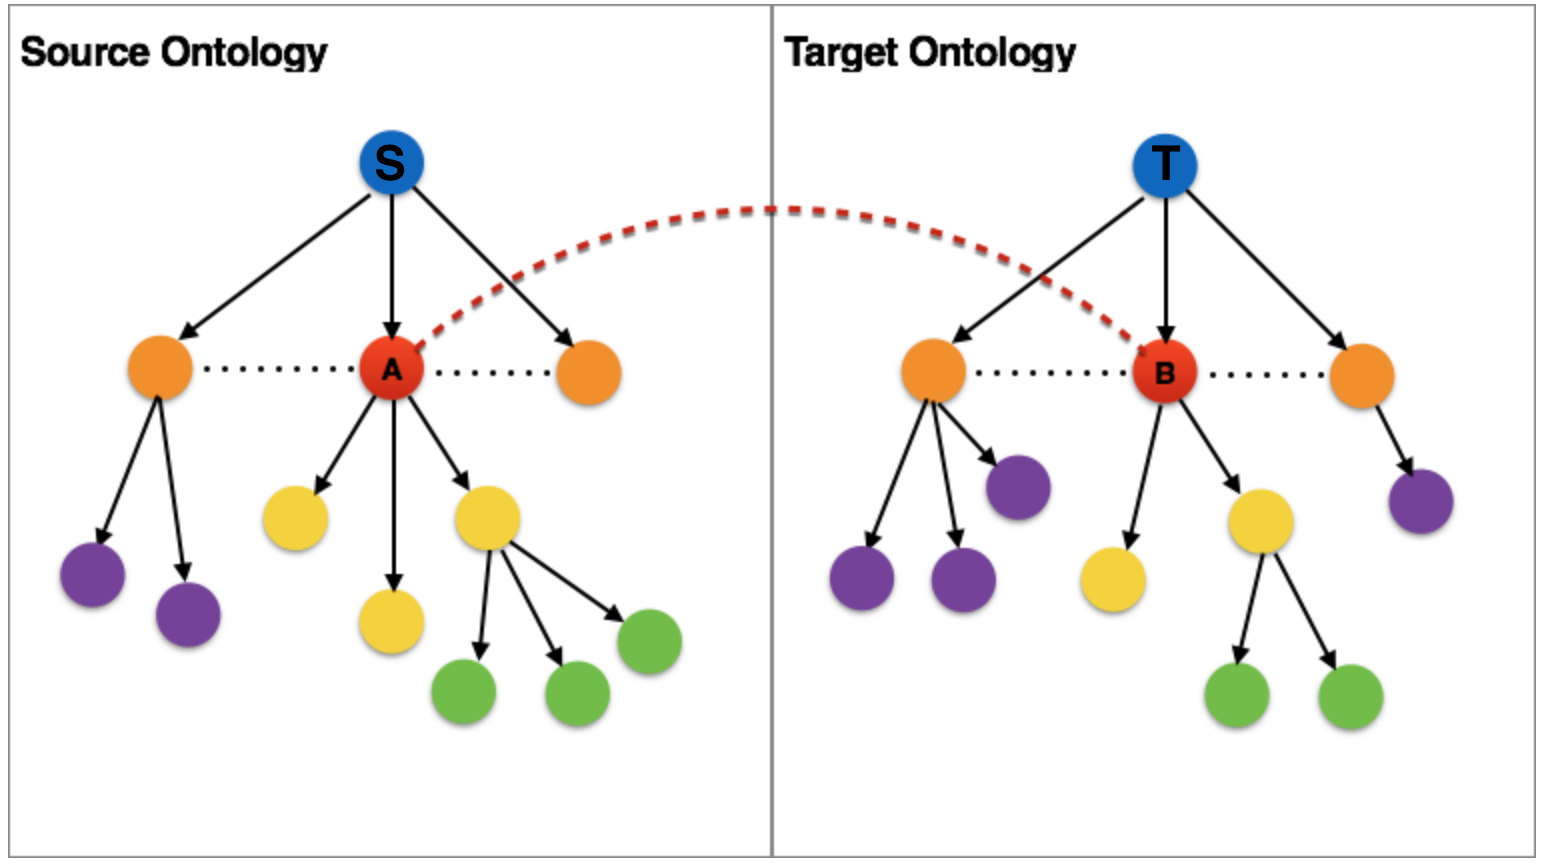
\includegraphics[width=3.5in]{pics/proto_tree.png}
	\caption{Two ontology subgraphs showing a mapping between nodes $A$
          and $B$.}
	\label{fig:proto_tree}
\end{figure}

% Besides the general information, we also provide detailed information about matching results and ontology structures. To deal with large ontology, we make use of the fact that users tend to pay more attention to structure-close ontology. So we only show the parent, children and siblings of the current node in view. This is clearly illustrated by Figure~\ref{fig:proto_tree}.

The next question we address from the interface viewpoint is how to
combine both types of navigation. %is how to combine the general and
                                %detailed view together. In order to
                                %let users easily see both two views, 
We provide a list that represents the children of a node and a tree
view that represents the siblings of the current node. 

\begin{figure*}[!ht]
	\centering
	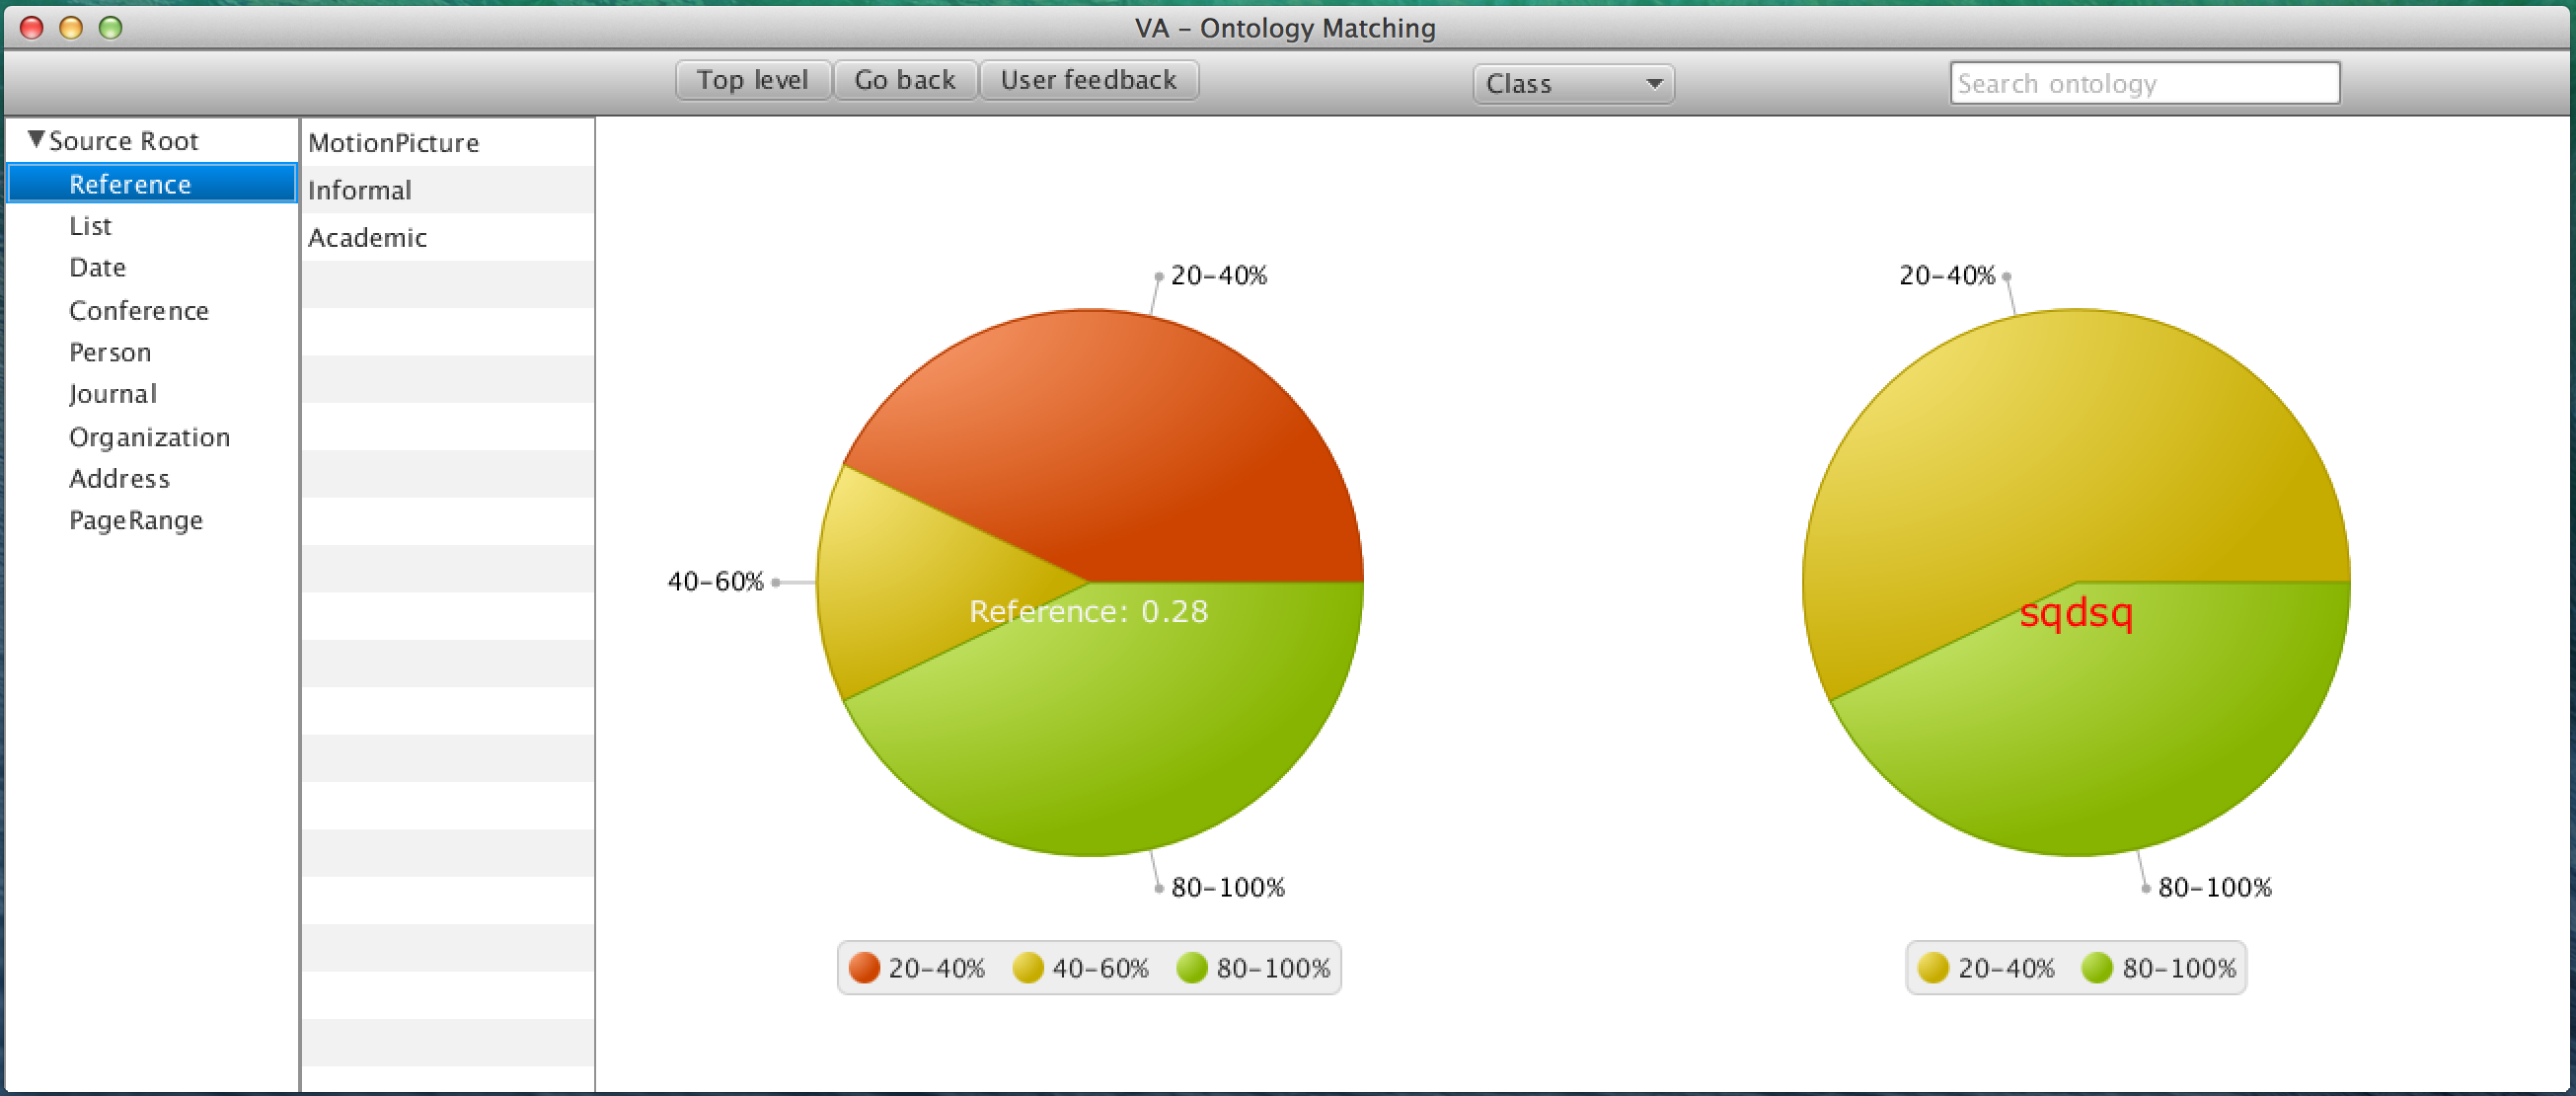
\includegraphics[width=6.5in]{pics/gui.png}
	\caption{Main panel.}
	\label{fig:main_panel}
\end{figure*}

The main panel of the user interface for the first version of the
prototype is shown in Figure~\ref{fig:main_panel}. In the center area
there are the two pie charts previously discussed. 

Immediately left of the pie charts there is a list. When the users click on a pie
chart slice, the list contains the ontology nodes with similarity
value within the corresponding range, ordered by that value. Clicking on a node in the list leads to an update of the
pie charts, as that node becomes the current node. The 
leftmost part of the interface contains the tree view. It shows all
the siblings of
the current node. When clicking on a node in the tree view, both the
pie charts and the lists will be updated, reflecting the change of the
current node. On the top right there is a
search box. Upon entering the name of the node in the search box, the
left pie chart will display that source node and the right pie chart
will display the target node that matches to the source
one. Accordingly, the tree and list view on the left will be updated as well. 
In addition, for an easier navigation we provide additional functions such as ``go
to the top level'', ``go to the previous level'', and ``switching
between class and property''. 

Upon entering the source ontology node's name in the search box and pressing the enter key on the keyboard, the left pie chart will display the source node that is searched and the right pie chart will display the target node that matches to the source one. Accordingly, the two lists on the left will be updated as well.

\section{Algorithm Comparison}

To compare the results of more than one matching algorithm, we need to
visualize their results at the same time. We have upgraded the main
panel to load  multiple results as shown in
Figure~\ref{fig:updated_main_panel}. %\marginpar{picture to be updated}


\begin{figure*}[!ht]
	\centering
	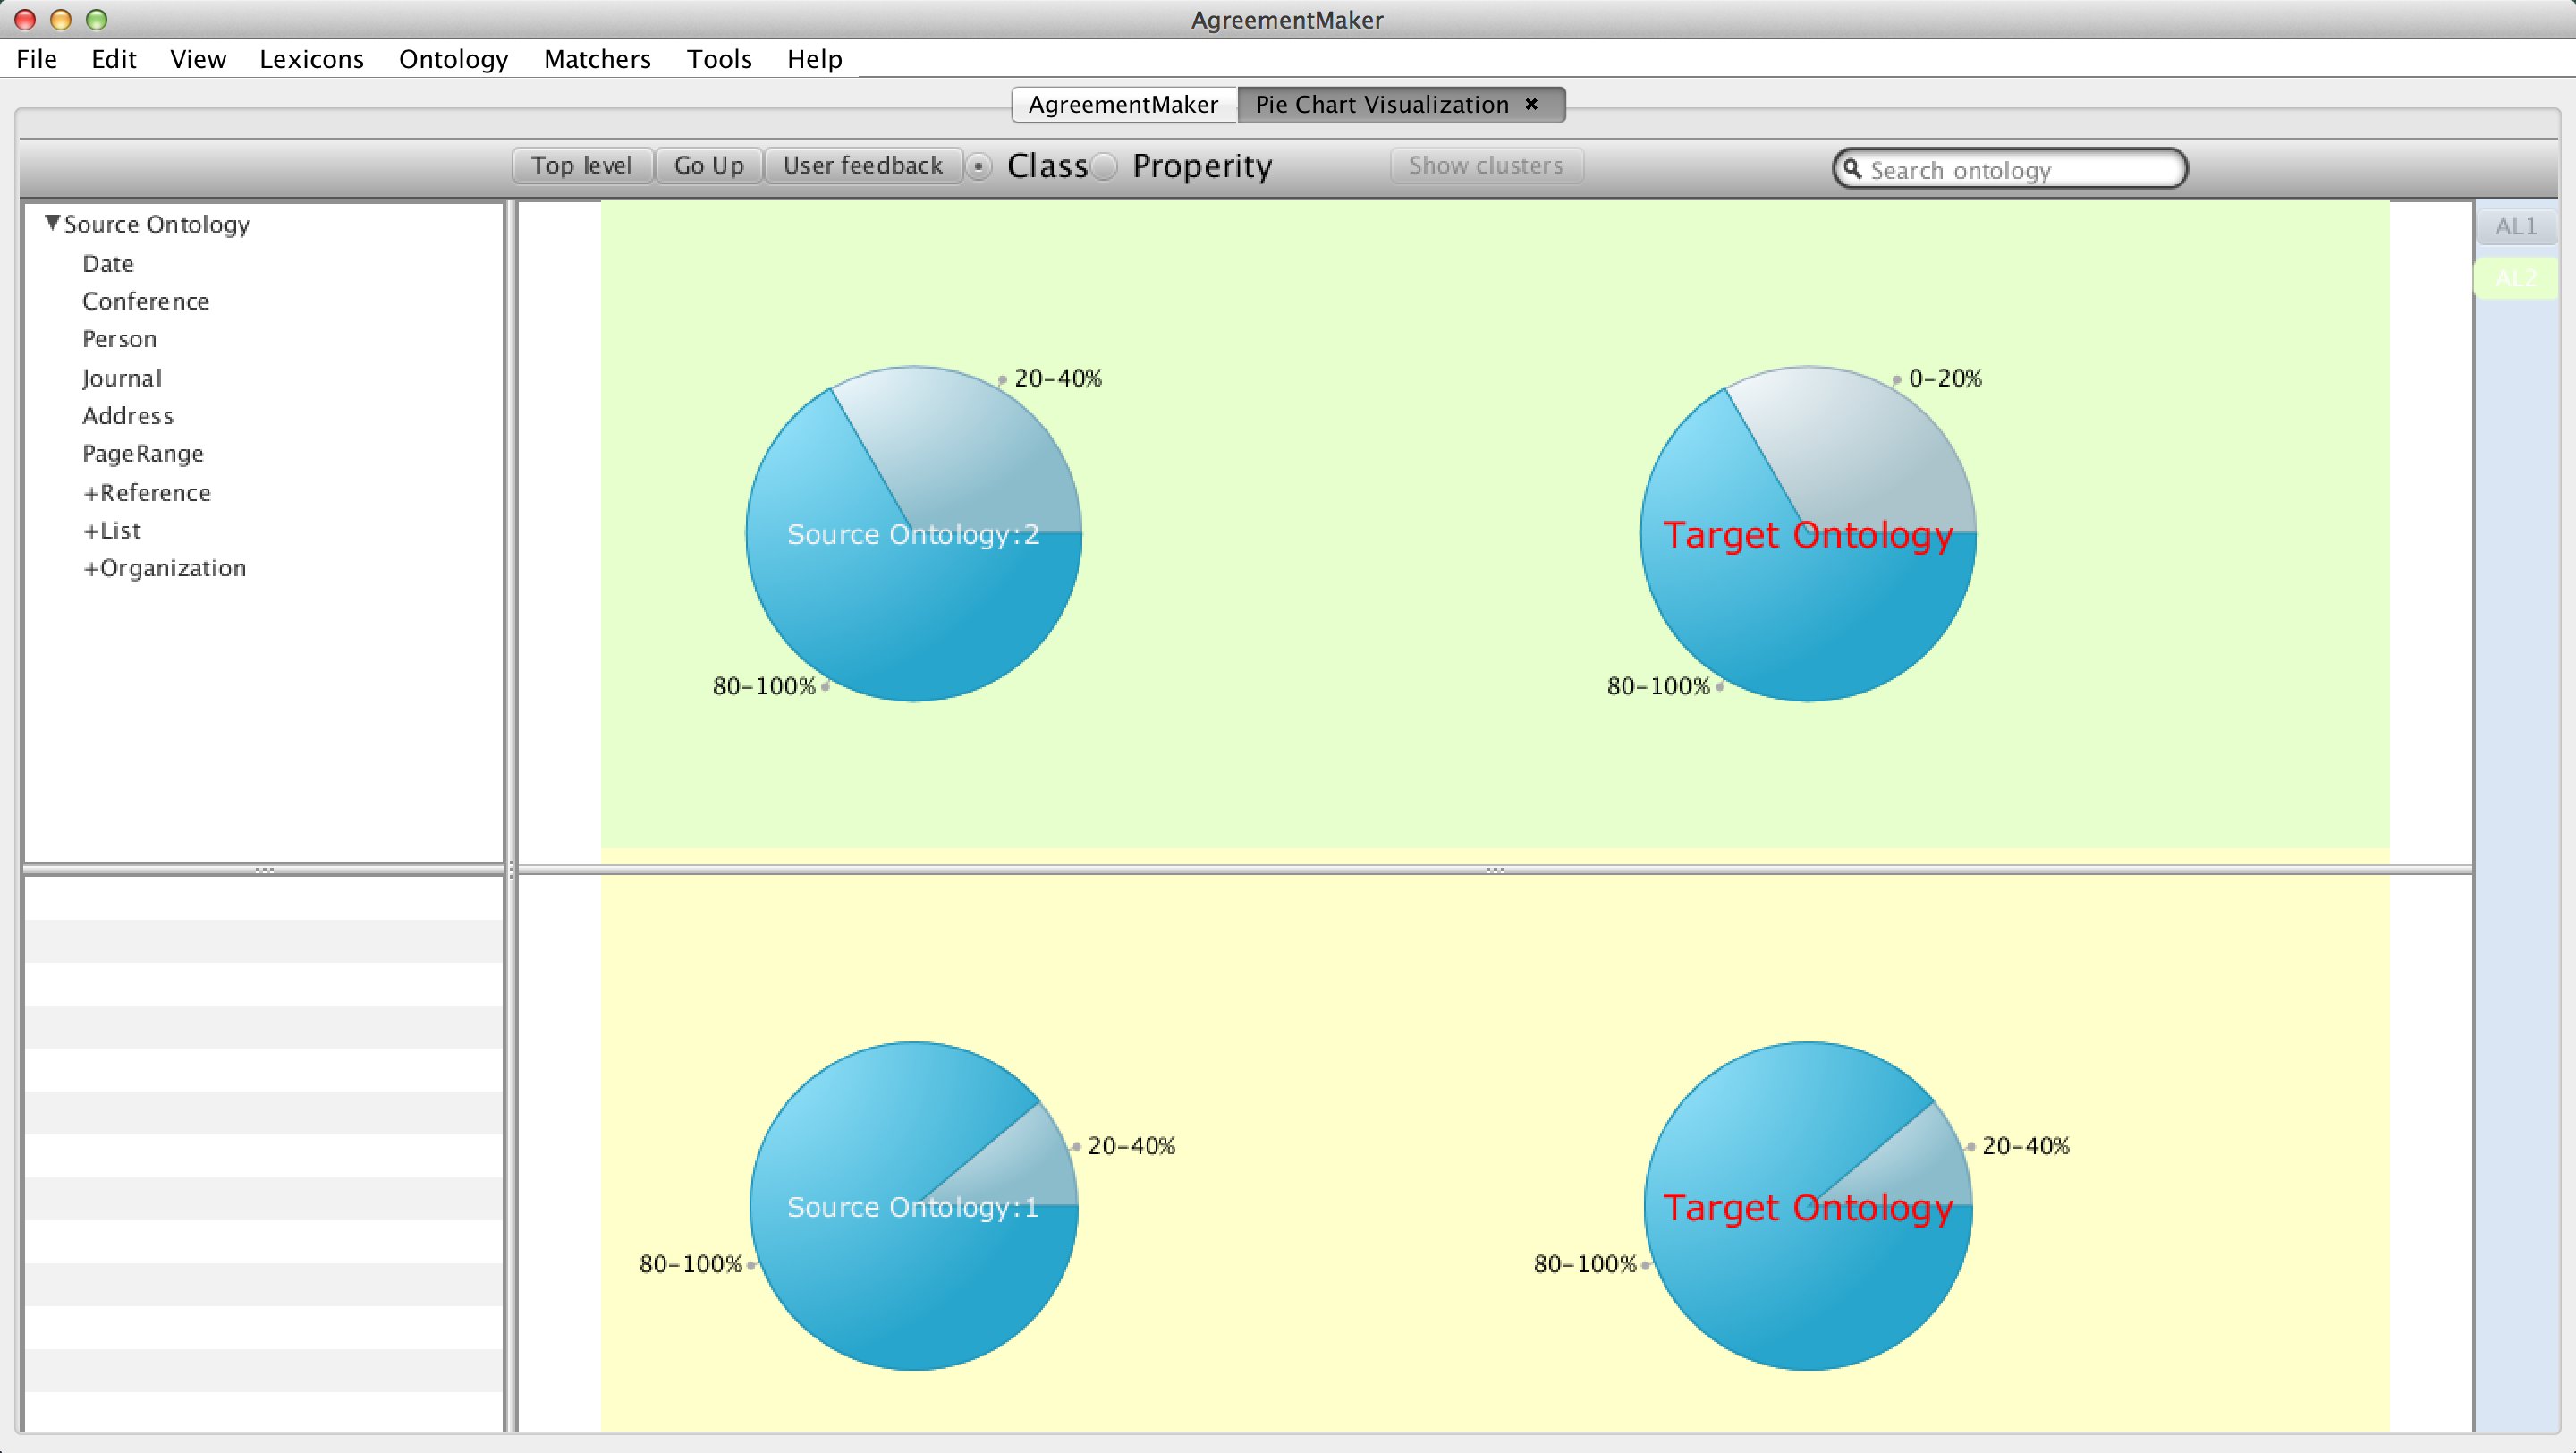
\includegraphics[width=6.5in]{pics/gui2.png}
	\caption{Updated main panel.}
	\label{fig:updated_main_panel}
\end{figure*}

We are making full use of the containers in JavaFX, in order to manage
the elements within the limited space. We use two tile panels to display two
sets of ontology pairs, the upper panel is the main panel and the
lower one is the sub panel. The tree view shows the siblings of the
source ontology in the main panel and the list view shows the children
nodes of that ontology. 

\begin{figure*}[!ht]
	\centering
	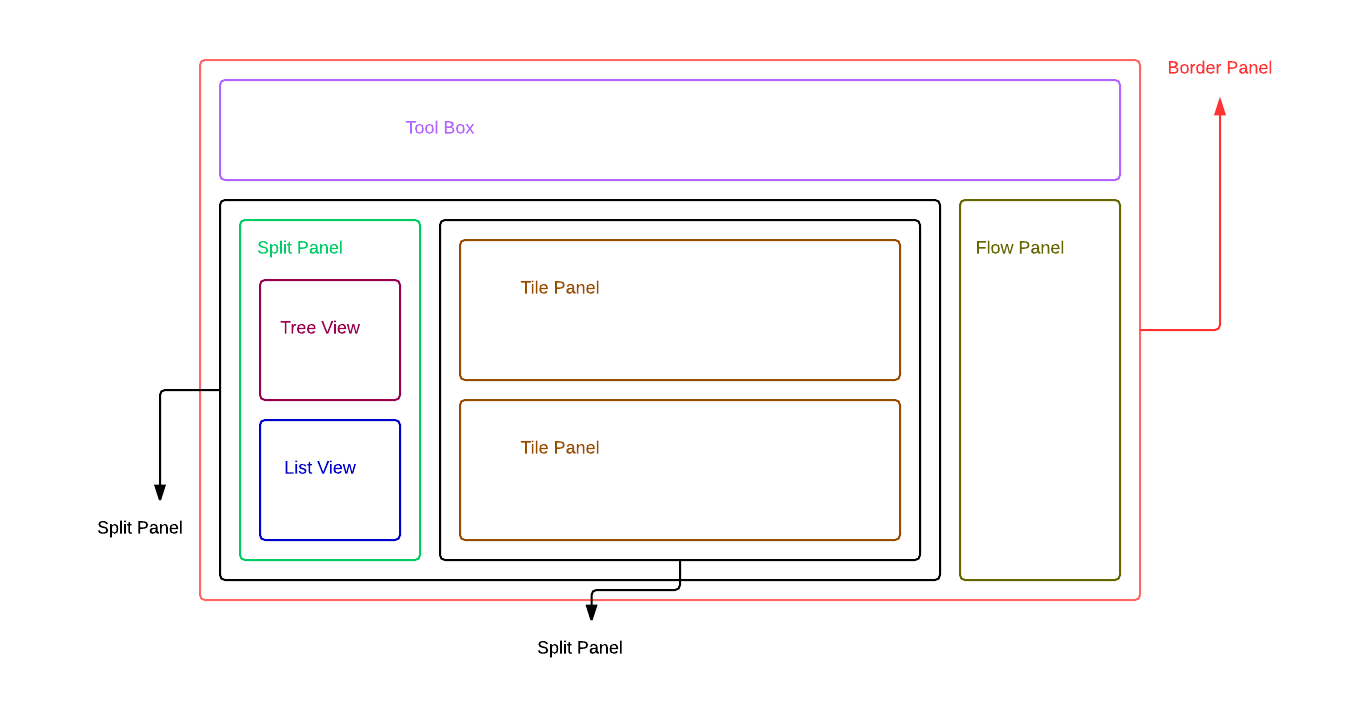
\includegraphics[width=6.5in]{pics/VA_UI.png}
	\caption{Graphical User Interface.}
	\label{fig:ui}
\end{figure*}

\section{Interaction with Multiple Ontologies} % (fold)
\label{sub:loading_multiple_ontology}

Figure~\ref{fig:ui} displays the organization of the user interface.
We divide the main panel into two sets. The top set in green is the
main set and the set below in yellow is the sub set. Each set has a
pair of source and target ontologies. The column bar on the rightmost
side shows the algorithms we have loaded into the application. The
main set shows the result of the second algorithm we load, which is
represented by the green button. The rest of the upgraded panel
remains the same as described previously.

In this way, we can choose any loaded algorithm to be the main set or
the sub set. The difference between the main set and the sub set is that
all lists get updated according to the changes to the main set. The reason for this design is that we have limited space on the screen panel and we need to choose the most significant information to display.

When the users click on the main set pie chart slice, all features
including all pie charts and the lists will be updated. To change the
matching algorithm of the main set, the users first click on the current main set algorithm button, then click on any other algorithm button to set it as the new main set.


%%=========================================
%\section{Graphic User Interface}
%We are making full use of the containers in JavaFX, in order to
%manage the elements within the limited space. See Figure~\ref{fig:ui}
%for the graphic user interface design. We use two tile panels to
%display two sets of ontology pairs, the upper panel is the main panel
%and the lower one is the sub panel. The tree view shows the siblings
%of the source ontology in the main panel and the list view shows the children nodes of a particular portion which user clicks on of the source ontology. 

